\chapter{COMPARACIÓN CON PYCLAW}
Se da una breve explicación del funcionamiento y diseño de la simulación del problema de condiciones iniciales del capítulo anterior con la librería PyClaw y se comparan los resultados obtenidos.


%
\begin{figure}[ht]
	\centering
	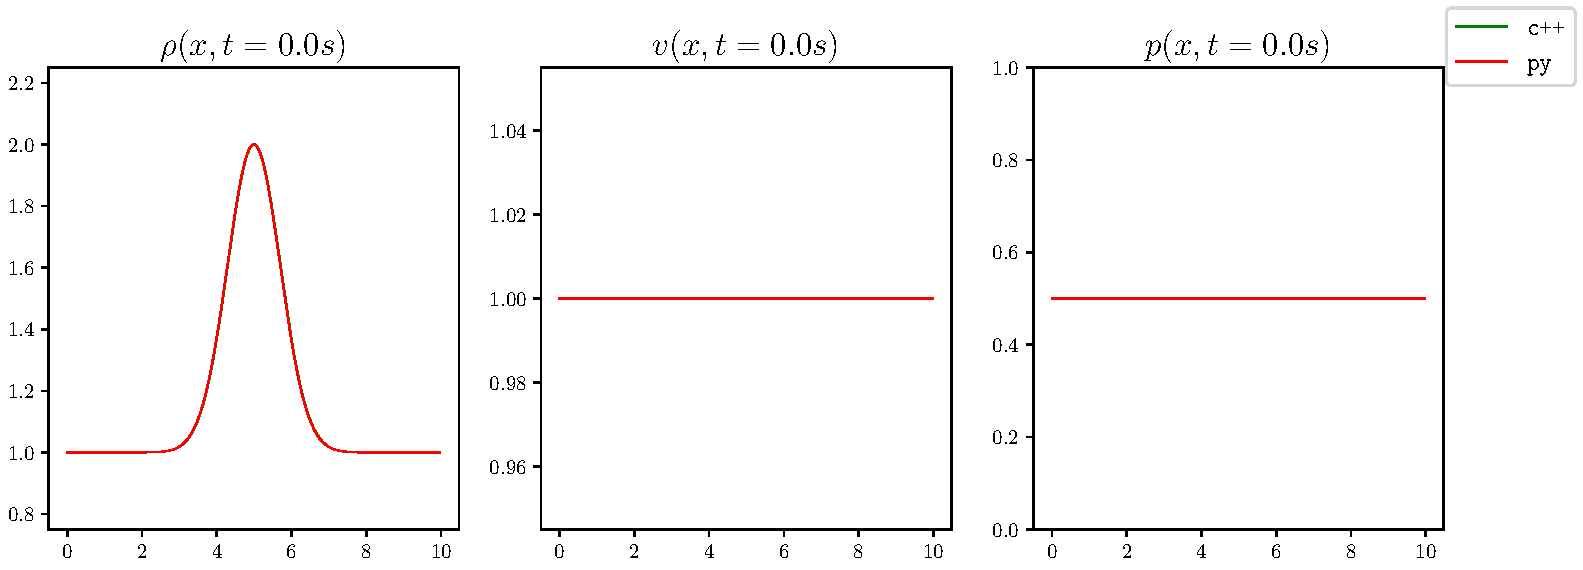
\includegraphics[width=1.1\linewidth]{../euler1D/plots_en_TDG/py_sin_claw/py_gauss199/1.pdf}
	\caption{Gráficas para $t=0.0\unit{\s}$}
\end{figure}
%C:\Users\Rodrigo\Documents\mundo9\Universo\tesis\euler1D\plots_en_TDG\py_sin_claw\py_gauss199\1.pdf